\section{Experiments and evaluation}
\label{sec:evaluation}
\subsection{Data and shared protocol}
\label{sec:protocol}
We ran the experiments on five standard benchmark databases from the FIM community:
Chess, Mushroom, Retail, T10I4D100K, and Accidents, all originally from the FIMI
repository~\cite{fimi}. Table~\ref{tab:datasets} lists statistics that we computed from
the data files themselves, where $N$ is the number of transactions, $|I|$ the number of
distinct items, $\bar{w}$ the mean transaction length, and the density
$d = \bar{w} / |I|$ the average fraction of items present in a transaction. Chess and
Mushroom are dense ($d \ge 0.19$), while Retail and T10I4D100K are sparse
($d \le 0.012$). Accidents has $d = 0.072$, between the two groups, but we group it with
the dense databases because of its long transactions ($\bar{w} = 33.81$, close to Chess),
which make its output grow as fast as theirs (Section~\ref{sec:output-size}).

\begin{table}[t]
\centering
\caption{Statistics of the five benchmarks, computed from SHA-256-checked files}
\label{tab:datasets}
\begin{tabular}{lrrrrr}
\hline
Data & $N$ & $|I|$ & $\bar{w}$ & $w_{\max}$ & $d$ \\
\hline
Chess & 3\,196 & 75 & 37.00 & 37 & 0.493 \\
Mushroom & 8\,124 & 119 & 23.00 & 23 & 0.193 \\
Retail & 88\,162 & 16\,470 & 10.31 & 76 & 0.0006 \\
T10I4D100K & 100\,000 & 870 & 10.10 & 29 & 0.0116 \\
Accidents & 340\,183 & 468 & 33.81 & 51 & 0.072 \\
\hline
\end{tabular}
\end{table}

We identify each file by its SHA-256 hash rather than by its name, because one name can
refer to several different versions. The \texttt{mushrooms.txt} file on the SPMF site has
8\,416 transactions, unlike the 8\,124-transaction FIMI version used by the assignment and
by most papers, so we use the FIMI version. Retail holds the anonymized receipts of a
Belgian retail store~\cite{brijs1999}, and Accidents holds records of traffic accidents
with injuries in Flanders, Belgium~\cite{geurts2003}. The SPMF copies of Chess and
Accidents are byte-identical to the FIMI ones. The FIMI versions of Retail and T10I4D100K
contain item 0, while SPMF accepts only positive integer items, so we use the SPMF
versions, in which every item code is shifted up by 1. This renaming keeps the support of
every itemset unchanged. The script \texttt{experiments/prepare\_benchmarks.jl}
downloads the data again and checks hashes and statistics before any file is used.

A relative minsup is converted to a transaction count
$\sigma = \lceil \mathrm{minsup} \cdot N \rceil$. During the experiments we found that
SPMF computes this product in 64-bit floating point, so with $\mathrm{minsup} = 0.07$ and
$N = 100$ SPMF requires $\sigma = 8$, while exact decimal arithmetic gives $\sigma = 7$.
The experiment runner therefore rejects every threshold where the two computations
disagree, so that any difference between the two implementations can only come from the
algorithm.

Every attempt runs in a fresh process with a timeout and is recorded as CSV rows with the
same set of fields: dataset and hash, minsup and $\sigma$, Git revision, algorithm
variant, environment, seed, time, peak memory, itemset count, and status. A failed or
timed-out attempt is kept with its status and is never replaced by a zero. Time is split
by timing scope. The \emph{process} scope measures the whole process, including Julia
start-up, JIT compilation, or JVM start-up. The \emph{mine} scope measures
only the call to \texttt{mine} after a warm-up run on a small database, so it contains no
compilation time. For SPMF we also record the time SPMF reports itself. Peak memory is the
peak RSS (Section~\ref{sec:measure}), as the operating system reports it through
\texttt{getrusage}, because only this quantity is comparable between a Julia process and a
Java process.

Every measurement in this paper ran on the grading machine: Linux, an Intel Core
i7-11800H with its clock fixed at 2.3\,GHz, 7.4\,GiB RAM, single-threaded Julia 1.13.2,
and the pinned SPMF release~\cite{spmf2016} on Java Temurin 25.0.4.1 with a 4\,GiB heap.

\subsection{Correctness and memory}
\label{sec:exact-memory}
\subsubsection{Comparison with SPMF}
Two implementations can produce the same number of itemsets but assign different
supports. We therefore use SPMF's Eclat as an independent reference and compare the full
map from itemset to support count. The comparator skips metadata lines and sorts the
items inside each key, so print order does not affect the result. The match rate is the
number of keys that appear exactly once on each side with the same support, divided by
the number of distinct keys in the union of the two outputs. Two empty maps count as a
full match. The report lists missing, extra, duplicate, and wrong-support keys
separately.

Table~\ref{tab:toy-spmf} shows the results on seven small databases. $N$ is the number
of transactions and $\sigma$ the support threshold in transactions, as in
Section~\ref{sec:protocol}. The ``Match'' column gives the number of itemsets with the
same support as SPMF over the total number of distinct itemsets. Every comparison of the
baseline reaches 100\%, with no missing, extra, duplicate, or wrong-support itemset. For
\texttt{disjoint}, both programs return an empty map. The \texttt{boundary} database runs
at two thresholds to check itemsets just above and just below the threshold. Each
threshold is chosen so that SPMF and exact decimal arithmetic give the same $\sigma$. The
test suite checks the stored SPMF outputs against every Eclat variant on every run.

\begin{table}[t]
\centering
\caption{Full itemset and support comparison of the baseline Eclat with SPMF on small
databases}
\label{tab:toy-spmf}
\begin{tabular}{lrrr}
\hline
Data & $N$ & $\sigma$ & Match \\
\hline
Baskets & 4 & 2 & 6/6 \\
Duplicates & 3 & 2 & 3/3 \\
Disjoint & 3 & 2 & 0/0 \\
Dense & 2 & 2 & 7/7 \\
Groceries & 5 & 2 & 5/5 \\
Boundary & 4 & 2 & 2/2 \\
Boundary & 4 & 1 & 4/4 \\
Nested & 4 & 2 & 3/3 \\
\hline
\end{tabular}
\end{table}

On the five benchmarks, we checked every output of the runtime campaign of
Section~\ref{sec:minsup}: both variants at revision \texttt{ca60f43}, five repeats at each
of 33 pairs of database and threshold, against one independent SPMF Eclat result per pair.
All 330 outputs of the two variants reach a 100\% match rate, with 0 missing, extra,
duplicate, or wrong-support itemsets. Table~\ref{tab:bench-exact} gives the number of
matching thresholds for each variant and the range of SPMF output sizes.
Fig.~\ref{fig:exact-grid} shows the minsup values that were checked.

\begin{figure}[t]
\centering
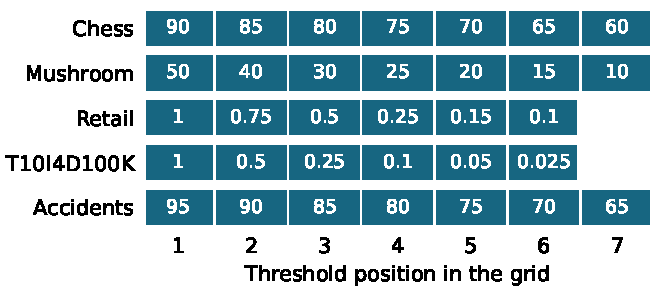
\includegraphics[width=\columnwidth]{figures/en/correctness-grid.pdf}
\caption{Minsup grid per database. Each cell gives minsup as a percentage and marks a
point where both variants match SPMF on every itemset and support.}
\label{fig:exact-grid}
\end{figure}

\begin{table}[t]
\centering
\caption{Thresholds whose full output matches SPMF, and the number of reference itemsets}
\label{tab:bench-exact}
\begin{tabular}{lrrr}
\hline
Data & Baseline & Optimized & Itemset range \\
\hline
Chess & 7/7 & 7/7 & 622--254\,944 \\
Mushroom & 7/7 & 7/7 & 153--574\,431 \\
Retail & 6/6 & 6/6 & 159--7\,589 \\
T10I4D100K & 6/6 & 6/6 & 385--96\,959 \\
Accidents & 7/7 & 7/7 & 15--1\,093 \\
\hline
\end{tabular}
\end{table}

\subsubsection{Process peak memory}
The same campaign records the peak RSS of every run. The measurement covers start-up,
reading the data, mining, and writing the whole output. Table~\ref{tab:peak-rss} gives
the medians at the lowest minsup of each database, where the output and the search are
largest. Every program reports at least 252\,MiB at every point, a floor set by the
measurement itself, so a value at that floor is only an upper bound.

\begin{table}[t]
\centering
\small
\setlength{\tabcolsep}{3pt}
\caption{Median peak RSS (MiB) over five repeats at the lowest minsup of each database.
$R$ is the baseline's median divided by the optimized variant's.}
\label{tab:peak-rss}
\begin{tabular}{lrrrrr}
\hline
Data / minsup & Baseline & Optimized & $R$ & SPMF & PrePost+ \\
\hline
Chess / 0.6 & 285.1 & 261.5 & 1.090 & 526.5 & $\le 254$ \\
Mushroom / 0.1 & 366.0 & 299.2 & 1.223 & 514.2 & $\le 254$ \\
Retail / 0.001 & 289.6 & 280.9 & 1.031 & 844.4 & $\le 254$ \\
T10I4D100K / 0.00025 & 303.7 & 278.5 & 1.090 & 556.0 & 297.4 \\
Accidents / 0.65 & 608.4 & 398.3 & 1.528 & 4\,248.1 & 340.9 \\
\hline
\end{tabular}
\end{table}

From the medians in the table, the percentage reduction is $100(1-M_o/M_b)$, where $M_b$
and $M_o$ are the median peak RSS of the baseline and the optimized variant. The reduction
ranges from 3.0\% on Retail to 34.5\% on Accidents. SPMF Eclat uses 1.7 to 10.7 times as
much as the optimized variant. PrePost+ uses less on Accidents (340.9 against
398.3\,MiB) and stays at the floor on Chess, Mushroom, and Retail. The optimized variant uses \emph{bitsets} (bit
arrays) and reuses buffers when it intersects tidsets in Eclat's prefix
search~\cite{zaki2000}. For a database of $N$ transactions, a tidset with $s$ tids takes
$8s$ bytes as a list of 64-bit integers and $8\lceil N/64\rceil$ bytes as a bit array,
counting elements only. The bit array saves space for long tidsets, and the optimized
variant can switch classes with short tidsets to lists. Peak RSS combines the data, the
search structures, the result, and the runtime's own memory. The numbers show the
whole-process difference at the chosen thresholds.

\subsection{Runtime, output size, and scalability}
\subsubsection{Runtime against minimum support}
\label{sec:minsup}
We timed four programs in a single session on the grading machine
(Section~\ref{sec:protocol}): the baseline, the optimized variant, SPMF 2.66 Eclat, and
SPMF PrePost+. Both Julia variants ran through the \texttt{demo.jl} command-line
interface at the same revision (\texttt{ca60f43}), so the times use the \emph{process}
scope: from process launch until the output file is written, including Julia or JVM
start-up, reading, and writing. The grid has 33 (benchmark, minsup) points on the five
benchmarks of Table~\ref{tab:datasets}, and each point was repeated five times. All 660
runs were checked itemset by itemset against an independent SPMF Eclat run and matched
exactly.

Each point is the median of its five repeats. The interquartile range relative to the
median is at most 2.9\% for the baseline and 1.9\% for the optimized variant at every
point. For SPMF and PrePost+ it reaches 11.3\% and 13.9\%, and only one SPMF point and
three PrePost+ points exceed 10\%. To estimate drift between sessions, we compared with
three other sessions on the same machine. The PrePost+ times (the same Java command) of
this session differ by $+3.0\%$, $+1.9\%$, and $-2.3\%$ in geometric mean, and by at most
14.4\% at a single point. The optimized variant measured in another session at the same
revision differs by $-1.5\%$ on average and at most 5.6\%. The four programs in the tables
ran in the same session, so a ratio between two of them carries only within-session
noise. We treat a ratio as a real difference when it exceeds the sum of the two largest
interquartile ranges: about 5\% between the two Julia variants and about 16\% when one
side is a Java program. Drift between sessions matters only when comparing with another
campaign, at 5.6\% for the optimized variant and 14.4\% for PrePost+.

\begin{figure*}[t]
\centering
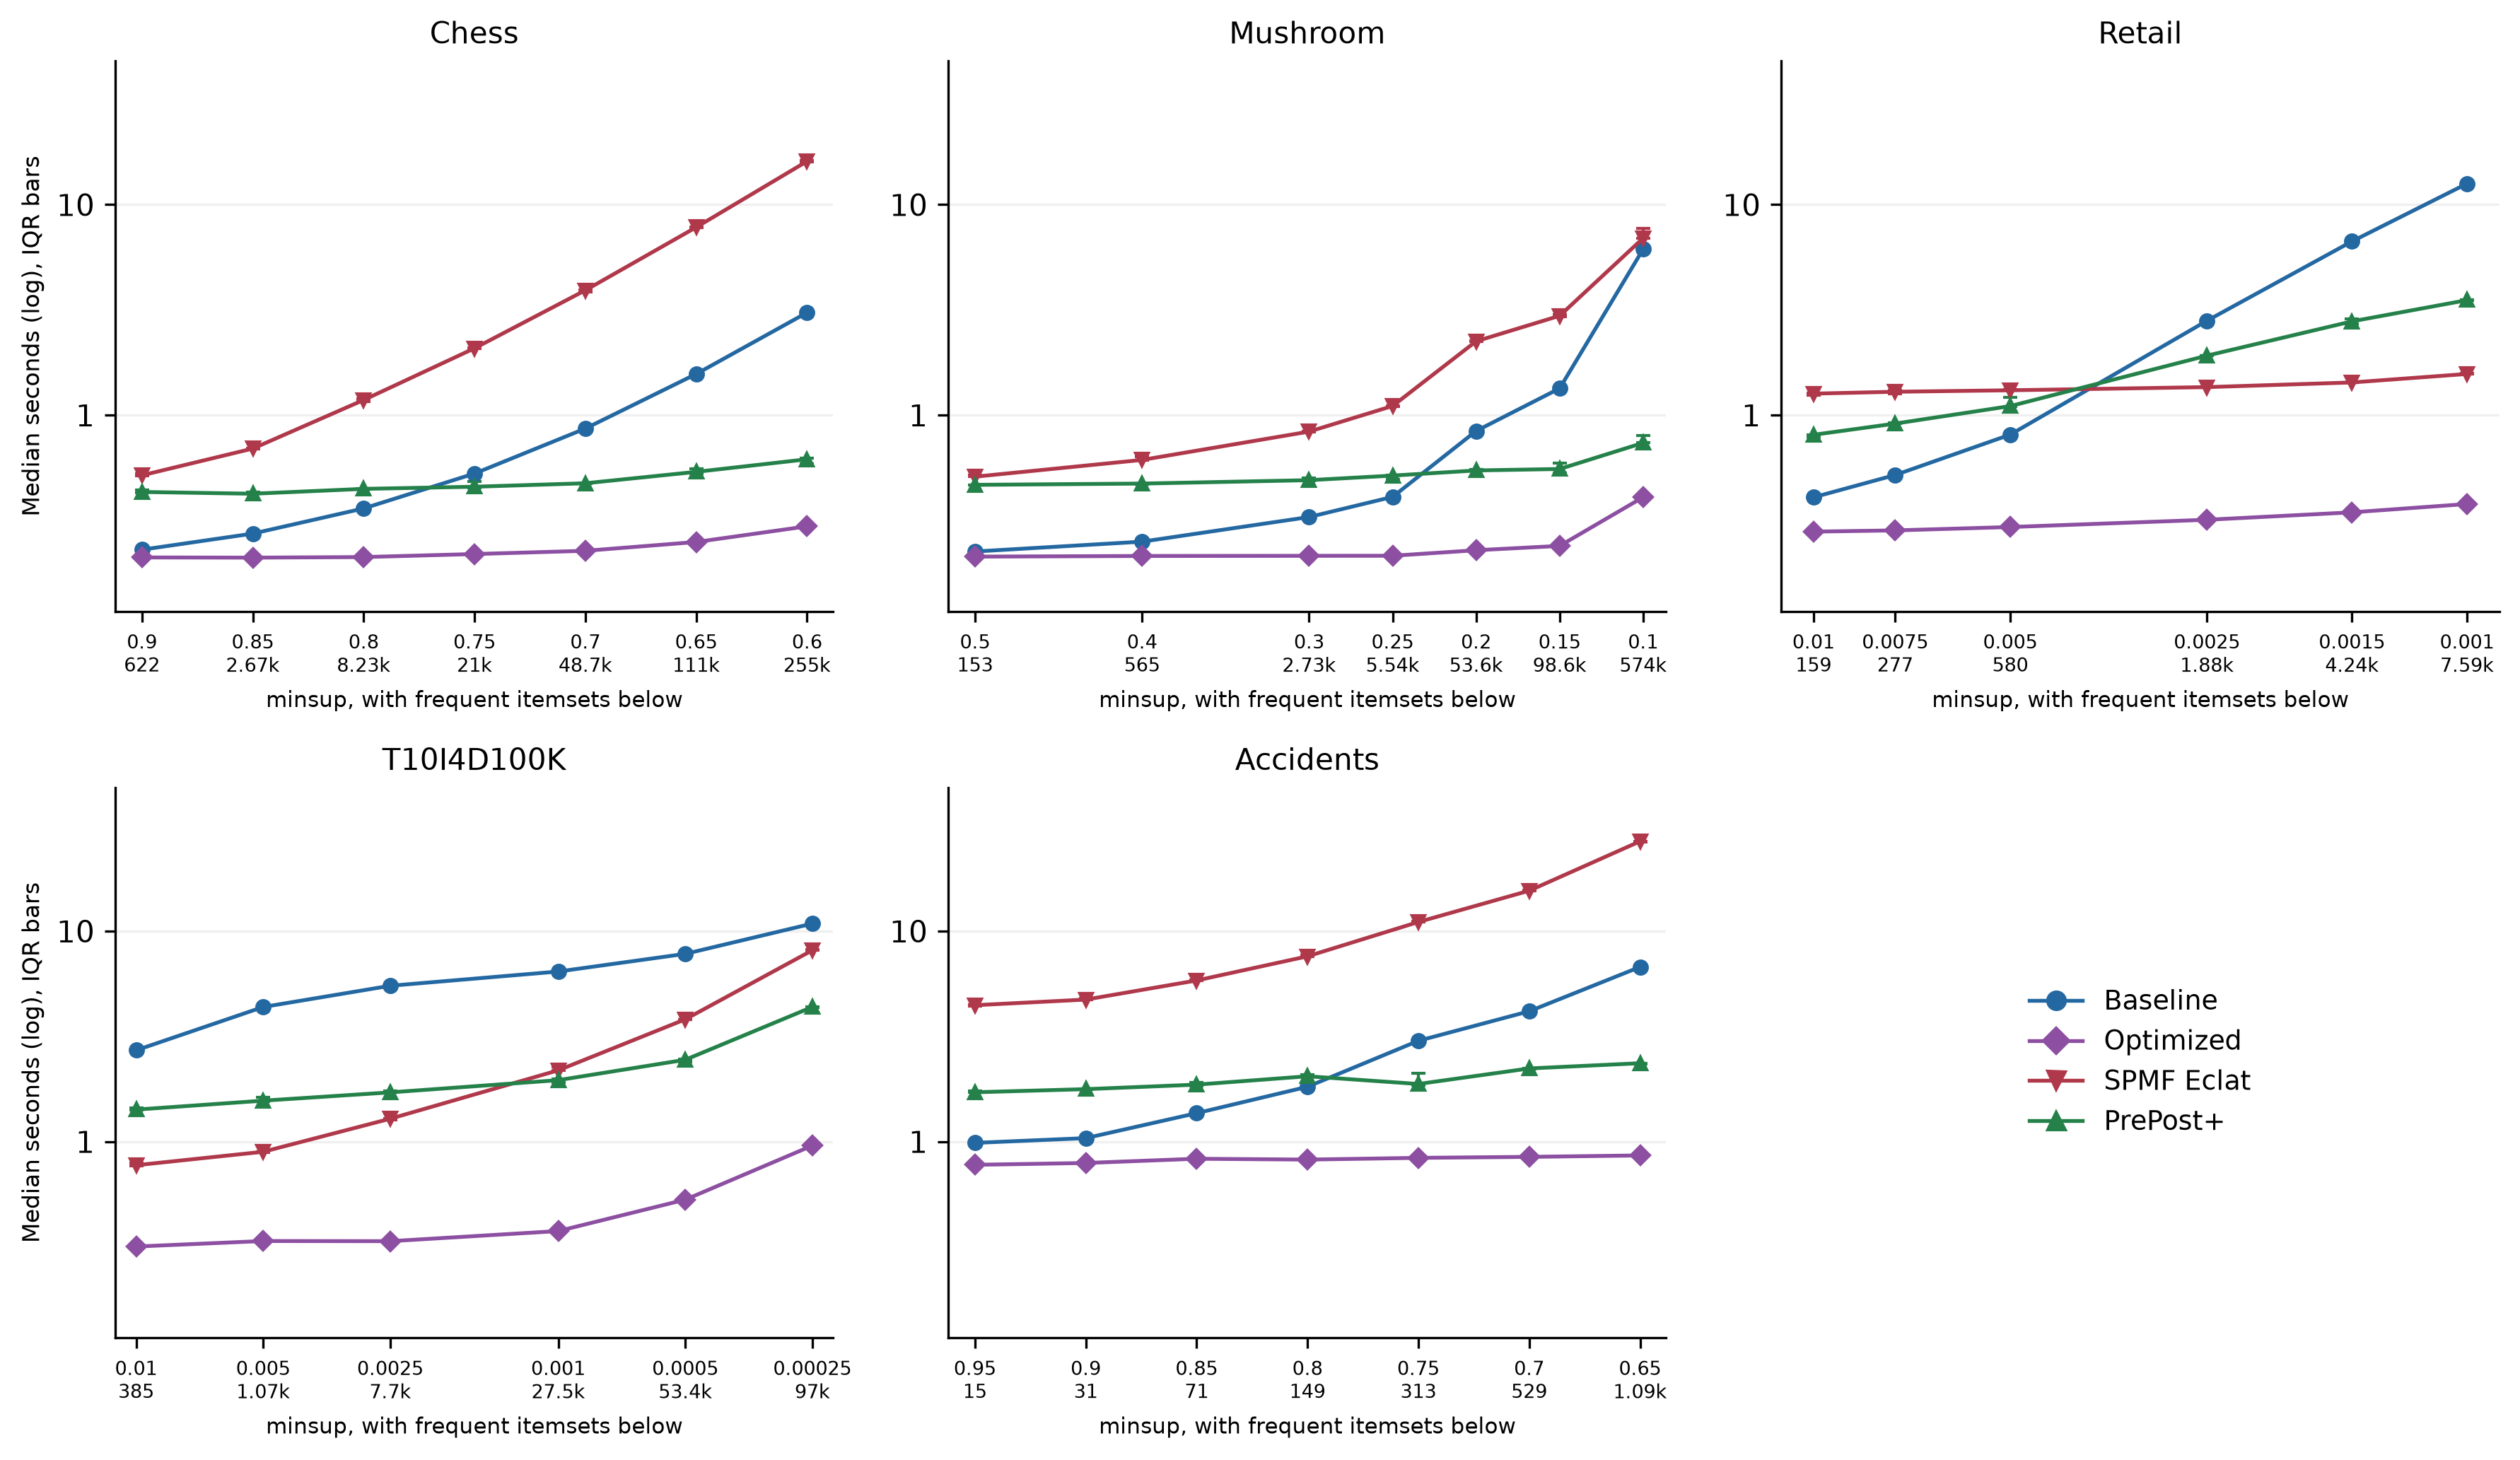
\includegraphics[width=\textwidth]{figures/runtime-curves.png}
\caption{\emph{Process} time against minsup for the four programs on the five
benchmarks. The vertical axis is logarithmic, points are medians of five repeats, and bars
are interquartile ranges. Below each horizontal-axis label is the number of frequent
itemsets.}
\label{fig:runtime}
\end{figure*}

The optimized variant is the fastest at all 33 points, at 0.21 to 0.96\,s. At the lowest
minsup of each benchmark (Table~\ref{tab:runtime-low}) it is faster than the baseline by
about 7.9 times on Accidents, 10.4 on Chess, 11.3 on T10I4D100K, 15.1 on Mushroom, and
33.3 on Retail. Table~\ref{tab:runtime-ratio} gives the geometric mean of this ratio over
every point of each benchmark, together with the ratios of SPMF Eclat and PrePost+ to the
optimized variant.

\begin{table}[t]
\centering
\footnotesize
\setlength{\tabcolsep}{3pt}
\caption{\emph{Process} time (seconds) at the lowest minsup of each benchmark, median of
five repeats. ``Sets'' is the number of frequent itemsets.}
\label{tab:runtime-low}
\begin{tabular}{lrrrrrr}
\hline
Data / minsup & Sets & Baseline & Optimized & SPMF & PrePost+ \\
\hline
Chess / 0.6 & 254\,944 & 3.07 & 0.30 & 16.07 & 0.62 \\
Mushroom / 0.1 & 574\,431 & 6.15 & 0.41 & 6.93 & 0.74 \\
Retail / 0.001 & 7\,589 & 12.59 & 0.38 & 1.57 & 3.52 \\
T10I4D100K / 0.00025 & 96\,959 & 10.86 & 0.96 & 8.11 & 4.36 \\
Accidents / 0.65 & 1\,093 & 6.76 & 0.86 & 26.70 & 2.36 \\
\hline
\end{tabular}
\end{table}

\begin{table}[t]
\centering
\small
\setlength{\tabcolsep}{4pt}
\caption{Geometric mean over every point of each benchmark of the \emph{process} time
ratio: the time of the program named in the column header divided by the time of the
optimized variant. A value above 1 means slower than the optimized variant.}
\label{tab:runtime-ratio}
\begin{tabular}{lrrr}
\hline
Data & Baseline & SPMF & PrePost+ \\
\hline
Chess & 2.83 & 10.33 & 2.08 \\
Mushroom & 2.73 & 6.01 & 2.22 \\
Retail & 5.89 & 4.34 & 5.01 \\
T10I4D100K & 13.14 & 4.53 & 4.76 \\
Accidents & 2.62 & 10.76 & 2.39 \\
\hline
\end{tabular}
\end{table}

The amount of work explains the shape of the baseline's curves. The baseline intersects
two sorted tidsets by merging them, so each intersection costs work proportional to the
combined length of the two tidsets. We reran the baseline's search on one thread and
counted the intersections (joins), the intersections that produced a frequent itemset,
and the combined length of the two tidsets over all intersections, which we call merged
elements (Table~\ref{tab:join-work}). Subtracting the time at the highest minsup (mostly
start-up and file reading) from the time at the lowest minsup and dividing by the
difference in merged elements, the baseline spends 2.0 to 6.9\,ns per element across the
five benchmarks. That is the same order as the 9.0 to 10.0\,ns from the transaction-length
experiment in Section~\ref{sec:width}.

\begin{table}[t]
\centering
\small
\setlength{\tabcolsep}{3pt}
\caption{Work done by the baseline at the lowest minsup of each benchmark. ``Success'' is
the share of intersections that produce a frequent itemset, ``Elements'' is the combined
length of the two tidsets over all intersections (billions), and ns/el is the time per
merged element after subtracting the time at the highest minsup.}
\label{tab:join-work}
\begin{tabular}{lrrrr}
\hline
Data / minsup & Joins & Success & Elements & ns/el \\
\hline
Chess / 0.6 & 326\,545 & 78.1\% & 1.43 & 2.0 \\
Mushroom / 0.1 & 722\,721 & 79.5\% & 1.66 & 3.6 \\
Retail / 0.001 & 3\,932\,582 & 0.14\% & 2.17 & 5.7 \\
T10I4D100K / 0.00025 & 4\,192\,075 & 2.3\% & 1.48 & 6.9 \\
Accidents / 0.65 & 2\,333 & 46.1\% & 1.22 & 4.8 \\
\hline
\end{tabular}
\end{table}

The structure of the data decides that work. On Chess and Mushroom, the number of
intersections is only 1.26 to 1.28 times the number of frequent itemsets and about 78\%
to 80\% of intersections succeed, so work grows with the number of frequent itemsets. On
Retail, minsup 0.001 produces 3.93 million intersections but only 5\,472 succeed, so each
frequent itemset costs about 286\,000 merged elements, and the baseline takes 12.59\,s,
8.0 times SPMF Eclat (1.57\,s) and 3.6 times PrePost+ (3.52\,s) at the same point. On
T10I4D100K, even minsup 0.01 needs 70\,127 intersections and 297.7 million merged
elements to produce exactly 10 two-item sets, so the baseline-to-optimized ratio is
already 8.5 at the first point. The optimized variant's curve is nearly flat and rises
clearly only at the points with the largest output (Mushroom 0.1, T10I4D100K 0.00025).
Section~\ref{sec:future} analyzes where the optimized variant spends its time.

At the highest minsup of Chess, Mushroom, Accidents, and Retail, the baseline-to-optimized
ratio is only 1.09, 1.06, 1.27, and 1.46. All four exceed the within-session noise
between the two Julia variants (about 5\%), so they are real differences, but small ones.
On Chess and Mushroom the gap is a few percent of a run that is mostly start-up and file
reading. On Accidents and Retail the absolute gap is only 0.21\,s and 0.13\,s, the same
order as start-up and file reading (about 0.21\,s on Chess at minsup 0.9, a point that
consists almost entirely of those steps). These ratios therefore do not show that the two
algorithms are equally fast. At the lowest minsup, SPMF Eclat is faster than the
baseline on Retail (8.0 times) and T10I4D100K (1.3 times) but slower on Chess (5.2 times)
and Accidents (4.0 times). On Mushroom, SPMF Eclat takes 6.93\,s and the baseline
6.15\,s. The 13\% gap is within the noise of a Java program (about 16\%), so the two
programs cannot be told apart. We treat SPMF as a black box, so we do not explain the
reversal at the other points.

These conclusions have limits: one machine, five repeats per point, and a
\emph{process} scope that includes Julia or JVM start-up (the Java programs also pay for
JVM start-up). The baseline is the version at revision \texttt{ca60f43}, which already
benefits from the faster reading and writing of later stages, so it is not the baseline
measured on 2026-10-31. The intersection counts come from a separate run, outside the
timed runs.

\subsubsection{Number of frequent itemsets against minsup}
\label{sec:output-size}
The output sizes come from the timing campaign of 2026-11-17 on 33 thresholds of the
five databases, shown in Fig.~\ref{fig:output-size}, so no extra mining was needed. That
campaign ran the baseline, the optimized variant, SPMF's Eclat, and PrePost+ five times
each at every threshold, and all 660 outputs match SPMF's Eclat exactly. The script
\texttt{scripts/output\_size.jl} checks three more properties on the kept outputs. First,
the four programs report the same number of itemsets at every threshold. Second, the
count never falls as minsup falls: by the anti-monotone property, every subset of a
frequent itemset is frequent, so lowering the threshold cannot lose an itemset. Third,
the outputs are nested: for each pair of adjacent thresholds $\sigma_1 > \sigma_2$, the
itemsets with support at least $\sigma_1$ in the output at $\sigma_2$ are exactly the
output at $\sigma_1$, with the same supports. Support does not depend on the threshold, so
this check catches a support that is wrong in only one run. All 28 threshold pairs
satisfy all three properties.

\begin{figure*}[t]
\centering
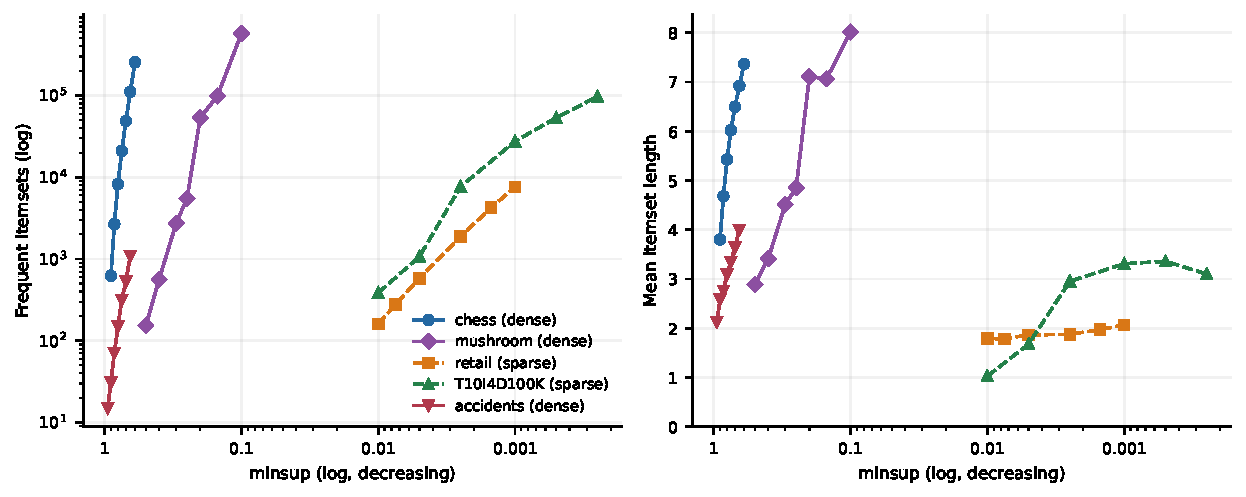
\includegraphics[width=\textwidth]{figures/en/output-size.pdf}
\caption{Number of frequent itemsets (left, log scale) and mean frequent-itemset length
(right) as minsup decreases on the five databases. Solid lines are dense data and dashed
lines are sparse data.}
\label{fig:output-size}
\end{figure*}

Fig.~\ref{fig:output-size} shows that the number of frequent itemsets grows much faster
on dense data. To compare growth rates across databases with different minsup ranges, we
fit the model
\begin{equation}
  \log F = c - s \log(\mathrm{minsup}),
  \label{eq:output-growth}
\end{equation}
where $F$ is the number of frequent itemsets at a threshold, $c$ is a per-database
constant, and $s$ is the slope on a log-log scale: when minsup falls by a factor $q$, $F$
grows by about $q^s$. Table~\ref{tab:output-growth} shows $s$ from 5.2 to 14.3 on the
three dense databases, but only 1.6 and 1.7 on the two sparse ones. Chess grows 410-fold
when minsup only drops from 0.9 to 0.6, while Retail grows 48-fold when minsup drops
tenfold.

\begin{table}[t]
\centering
\small
\caption{Number of frequent itemsets $F$ at the highest and lowest threshold, slope $s$
of model~\eqref{eq:output-growth}, and maximum frequent-itemset length $k_{\max}$ at the
lowest threshold}
\label{tab:output-growth}
\setlength{\tabcolsep}{4pt}
\begin{tabular}{lrrrrr}
\hline
Data & minsup & $F$ high & $F$ low & $s$ & $k_{\max}$ \\
\hline
Chess & 0.9--0.6 & 622 & 254\,944 & 14.3 & 14 \\
Accidents & 0.95--0.65 & 15 & 1\,093 & 11.3 & 8 \\
Mushroom & 0.5--0.1 & 153 & 574\,431 & 5.2 & 16 \\
Retail & 0.01--0.001 & 159 & 7\,589 & 1.7 & 5 \\
T10I4D100K & 0.01--0.00025 & 385 & 96\,959 & 1.6 & 11 \\
\hline
\end{tabular}
\end{table}

Itemset length explains the difference. In dense data, each transaction contains a large
share of the items, so many items occur together in most transactions and form long
frequent itemsets. A frequent $k$-itemset brings $2^k - 1$ non-empty subsets that are also
frequent, so whenever a lower threshold admits longer itemsets, the count grows
exponentially in their length. Mean length on Chess rises from 3.8 to 7.4 and on
Mushroom from 2.9 to 8.0 across the threshold grid. Mushroom grows 9.7-fold, from 5\,545
to 53\,583 itemsets, when minsup drops from 0.25 to 0.2, and at that same step the
maximum length rises from 11 to 15. In sparse data, transactions are short and items
rarely occur together, so lowering the threshold mostly adds single items and pairs. Mean
length on Retail stays between 1.8 and 2.1. On T10I4D100K 0.00025, 45\,660 of the 96\,959
itemsets, or 47\%, are 2-itemsets.

The number of frequent itemsets does not decide runtime on its own. In the same campaign,
the baseline takes 12.59 s on Retail 0.001 with 7\,589 itemsets, but only 3.07 s on
Chess 0.6 with 254\,944 itemsets. By~\eqref{eq:cost}, the cost is the number of
intersections times tidset length, not the number of results. Retail has 2\,117 frequent
items, so the root class has over two million pairs to intersect, and most of those
intersections fail without producing any itemset (Section~\ref{sec:optimized}). The
optimized variant avoids most of these intersections by counting pairs and runs Retail
0.001 in 0.38 s. Even with the optimized variant, Mushroom 0.1 with 574\,431 itemsets
takes 0.41 s, while T10I4D100K 0.00025 with 96\,959 itemsets takes 0.96 s, because
T10I4D100K's tidsets span 100\,000 transactions and most intersections at depth 2 fail.
The count dominates runtime only when it is very large: on Mushroom 0.05, before radix
sort, sorting and writing 3\,755\,511 itemsets took 89\% of the time and mining only 11\%
(Section~\ref{sec:optimized}). Conversely, when relative minsup is fixed, the count barely
changes, and runtime grows with $N$, as Section~\ref{sec:scalability} shows.

\subsubsection{Effect of transaction length}
\label{sec:width}
To separate transaction length from the density and output volume that are mixed together
in real benchmarks, we generated eight synthetic databases with the same $N = 10\,000$
transactions and $|I| = 100$ items, differing only in transaction length
$w \in \{5, 10, \dots, 40\}$. In the sampling model, each transaction is a uniformly random
subset of exactly $w$ items, independent of the other transactions, so the items are
interchangeable and no pair occurs together more often than chance. A $k$-itemset
therefore has expected support $N \prod_{j=0}^{k-1} (w - j)/(|I| - j)$; for example, a
pair appears in $N\,w(w-1)/(|I|(|I|-1))$ transactions. The generator uses SplitMix64 with
seed $(42 \ll 32) \,|\, w$ instead of Julia's \texttt{Xoshiro}, because Julia does not
guarantee the same random stream across versions. This keeps the SHA-256 hashes in the
manifest valid on every platform.

Two confounding factors need separating. The first is output volume: longer transactions
push more pairs and triples over the threshold, so the number of frequent itemsets grows
in steps, and runtime follows that count rather than necessarily following $w$. The second
is co-occurrence. The model removes it by keeping items independent, so the results
cannot stand in for the behavior of Chess or Mushroom. We therefore measure under two
protocols. The fixed protocol uses $\mathrm{minsup} = 0.05$ at every $w$. The
matched-output protocol uses, for each $w$, the largest threshold $\sigma$ that still
gives at least 5\,000 frequent itemsets, so output stays nearly constant and $w$ is the
only thing that changes.

Under the fixed protocol, the number of frequent itemsets is 53, 100, 100, 100, 5\,050,
5\,050, 5\,050, and 166\,749 as $w$ grows from 5 to 40. Pairs start to reach
$\sigma = 500$ at $w = 25$ (expected support 606, against 384 at $w = 20$), and triples at
$w = 40$ (expected 611). The baseline Eclat's runtime follows these steps (1.0\,s at
$w = 20$, 2.9\,s at $w = 25$, 49.4\,s at $w = 40$ in the \emph{process} scope,
Fig.~\ref{fig:width}), so a plot against $w$ at one minsup mostly reflects output, not
transaction length.

\begin{figure*}[t]
\centering
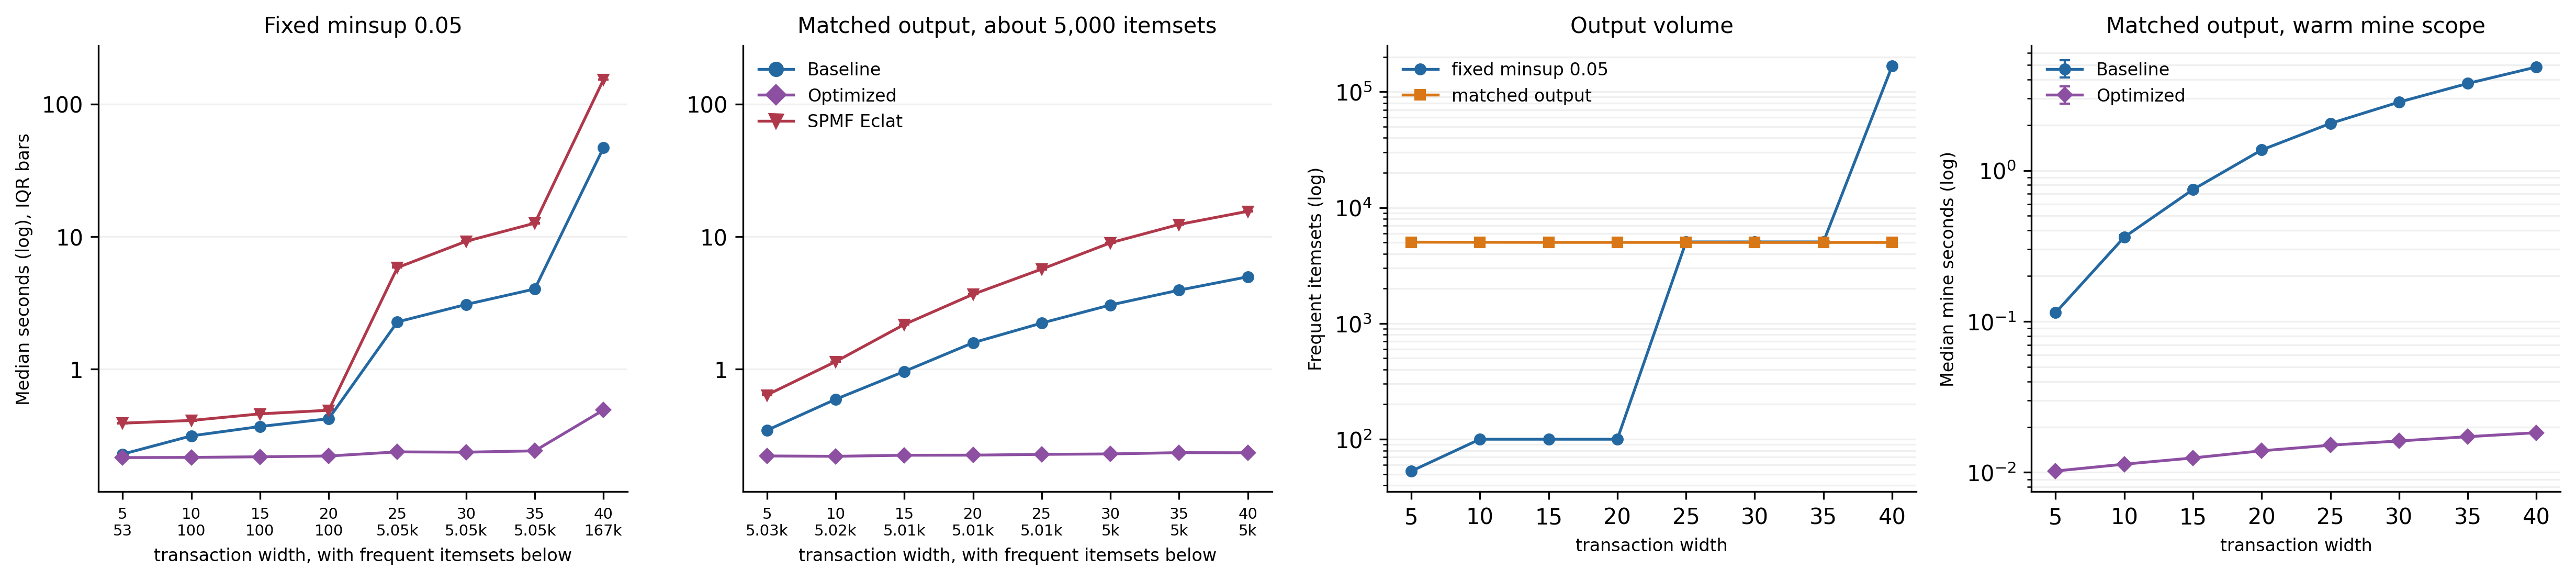
\includegraphics[width=\textwidth]{figures/width-curves.png}
\caption{Runtime and output volume against transaction length $w$ on the synthetic
databases ($N = 10\,000$, $|I| = 100$). From left to right: \emph{process} time at fixed
minsup 0.05; \emph{process} time with output matched to about 5\,000 itemsets; number of
frequent itemsets under both protocols; \emph{mine} time (after warm-up) with matched
output. Medians of three repeats with interquartile-range bars; below each axis label is
the number of frequent itemsets.}
\label{fig:width}
\end{figure*}

Under the matched-output protocol, the number of frequent itemsets stays around 5\,000 and
the number of tidset intersections (joins) is nearly constant (about 164\,000, of which
about 4\,900 succeed), but the baseline Eclat's mining time grows 42-fold as $w$ goes from
5 to 40 (Table~\ref{tab:width}). The reason is that the baseline intersects two sorted
tidsets by merging them, so each intersection costs work proportional to their combined
length. Each item appears in a fraction $w/|I|$ of the transactions, so its tidset length
is proportional to $w$, and the tidset of a pair is proportional to $w(w-1)$. The total
number of merged elements grows 47-fold while $w$ grows only 8-fold, and the baseline's
time tracks it at 9.0 to 10.0\,ns per element. The optimized variant intersects bitsets of
$\lceil N/64 \rceil = 157$ machine words regardless of tidset length, so its mining time
grows only 1.8-fold, from 10.2 to 18.3\,ms. In the \emph{process} scope, the optimized
variant is nearly flat at 0.79 to 0.80\,s because Julia start-up and compilation dominate.
We have not identified the source of that 1.8-fold growth. Under both protocols every
output matches SPMF exactly.

\begin{table}[t]
\centering
\caption{Eclat under the matched-output protocol. $\sigma$ is the threshold in
transactions, ``Elements'' is the combined length of the two tidsets over all of the
baseline's intersections, and times are \emph{mine} medians of three repeats.}
\label{tab:width}
\begin{tabular}{rrrrrr}
\hline
$w$ & $\sigma$ & Sets & Elements (M) & Baseline (s) & Optimized (ms) \\
\hline
5 & 10 & 5\,028 & 11.4 & 0.114 & 10.2 \\
10 & 69 & 5\,016 & 38.9 & 0.361 & 11.3 \\
15 & 179 & 5\,007 & 82.4 & 0.747 & 12.5 \\
20 & 340 & 5\,007 & 142.0 & 1.366 & 13.9 \\
25 & 550 & 5\,007 & 217.2 & 2.046 & 15.1 \\
30 & 815 & 5\,002 & 308.8 & 2.833 & 16.2 \\
35 & 1\,127 & 5\,002 & 416.4 & 3.765 & 17.2 \\
40 & 1\,488 & 5\,001 & 538.8 & 4.841 & 18.3 \\
\hline
\end{tabular}
\end{table}

As for the search tree, with minsup fixed the tree both deepens by one level at $w = 25$
(pairs) and $w = 40$ (triples) and widens: the number of intersections grows from 4\,950
to 166\,650 and then 4\,087\,798. With output matched, the tree has the same size at every
$w$, so only the cost per intersection changes. The scope of these conclusions is
limited: one $N$ and one item count, eight values of $w$, independent items, three
repeats on one machine, and a target of 5\,000 itemsets that is a choice, not a
derived value.

\subsubsection{Scalability}
\label{sec:scalability}
This experiment asks whether runtime grows linearly or nonlinearly with the number of
transactions $N$ when the database grows and the relative threshold stays fixed. We chose
Accidents, the largest database in Table~\ref{tab:datasets}, and Retail, the sparse
database with the most items. Each database was shuffled once with seed 42, and the $p\%$
subset holds the first $p\%$ of transactions of that permutation, with
$p \in \{10, 25, 50, 75, 100\}$. The subsets are therefore nested: a larger subset only
adds transactions and never replaces those of a smaller one, so the difference between two
points comes only from the added data. The script \texttt{experiments/prepare\_subsets.jl}
regenerates the subsets, and the SHA-256 hash of each file is recorded in
\texttt{data/benchmark/subsets.toml}. Mean transaction length barely changes between
subsets, from 33.79 to 33.81 on Accidents and from 10.30 to 10.37 on Retail, so sampling
does not change the shape of the data.

The threshold stays at minsup 0.65 for Accidents and 0.001 for Retail, the lowest
thresholds of each database in the runtime grid. The absolute threshold therefore grows
with $N$, from $\sigma = 22\,112$ to $221\,119$ on Accidents and from 9 to 89 on Retail.
The four programs were timed through the command line, each run in a fresh process, with
five interleaved repeats.
All 200 outputs match an independent SPMF Eclat run exactly. The interquartile range stays
within 1.9\% of the median for our two variants and 7.6\% for the two SPMF programs.

\begin{figure*}[t]
\centering
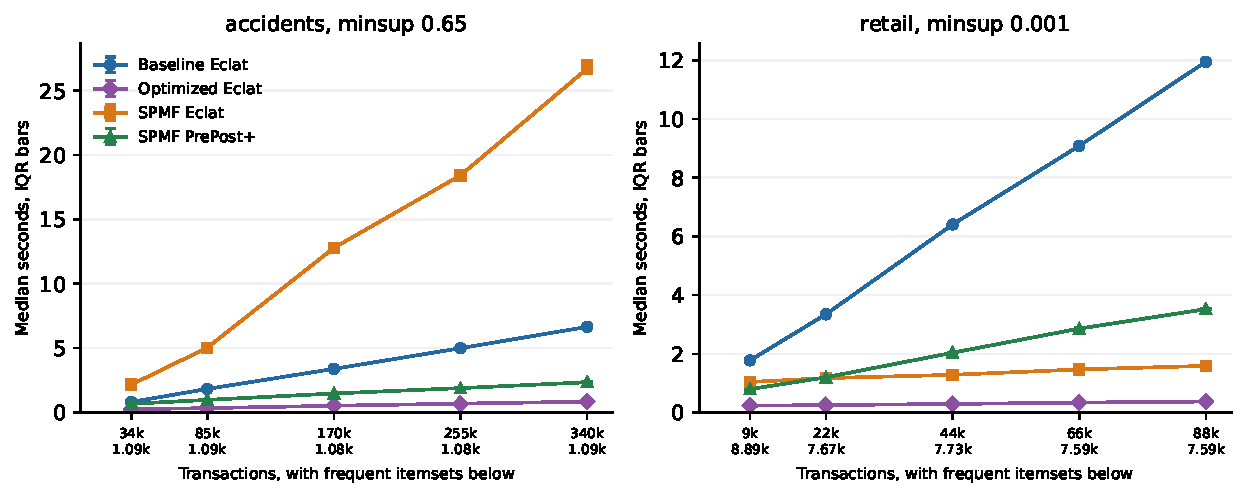
\includegraphics[width=\textwidth]{figures/en/scalability.pdf}
\caption{Median process time against number of transactions on five nested subsets of
Accidents (minsup 0.65) and Retail (minsup 0.001); error bars are the interquartile range
of five runs. The second row of numbers under the horizontal axis is the number of
frequent itemsets in each subset.}
\label{fig:scalability}
\end{figure*}

Fig.~\ref{fig:scalability} shows that all eight lines are close to straight. To check,
we fit each line with the model
\begin{equation}
  T(N) = a + b\,N,
  \label{eq:linear-fit}
\end{equation}
where $T(N)$ is the median time (seconds) on the subset with $N$ transactions, $a$ is a
fixed cost that does not depend on the data, and $b$ is the marginal cost per transaction.
The coefficient of determination $R^2$ is the share of the variance of $T$ that the model
explains, equal to 1 when the five points lie exactly on a line.
Table~\ref{tab:scalability-fit} shows $R^2 \ge 0.992$ for every line, so within the
measured range the runtime of all four programs grows linearly with $N$.

\begin{table}[t]
\centering
\small
\caption{Coefficients of model~\eqref{eq:linear-fit}: fixed cost $a$ (s), marginal cost
$b$ (s per 100\,000 transactions), coefficient of determination $R^2$, and the time ratio
between the 100\% and 10\% subsets}
\label{tab:scalability-fit}
\setlength{\tabcolsep}{4pt}
\begin{tabular}{llrrrr}
\hline
Data & Program & $a$ & $b$ & $R^2$ & $T_{100}/T_{10}$ \\
\hline
Accidents & Baseline & 0.19 & 1.90 & 0.9999 & 8.1 \\
 & Optimized & 0.19 & 0.20 & 0.9986 & 3.3 \\
 & SPMF Eclat & $-1.16$ & 8.02 & 0.9951 & 12.3 \\
 & PrePost+ & 0.52 & 0.54 & 0.9987 & 3.5 \\
Retail & Baseline & 0.61 & 12.87 & 0.9996 & 6.7 \\
 & Optimized & 0.22 & 0.18 & 0.9978 & 1.6 \\
 & SPMF Eclat & 1.00 & 0.69 & 0.9923 & 1.5 \\
 & PrePost+ & 0.48 & 3.51 & 0.9983 & 4.4 \\
\hline
\end{tabular}
\end{table}

The complexity analysis~\eqref{eq:cost} explains this trend. When relative minsup is
fixed, the set of frequent itemsets barely changes: Accidents has 1\,079 to 1\,095 frequent
itemsets at all five sizes. The equivalence classes visited are therefore the same, so the
number of intersections $C$ is nearly constant. Meanwhile the total length $L$ grows in
proportion to $N$, and each intersection costs time proportional to tidset length, which
is also roughly proportional to $N$, because a random sample keeps the share of
transactions that contain each itemset nearly the same. With bitsets, an intersection
reads $\lceil N/64 \rceil$ machine words, so the conclusion holds. All three terms are
linear in $N$, and no step of Eclat depends on the square of the number of transactions.

The fixed cost $a$ of the optimized variant is 0.19 s on Accidents and 0.22 s on Retail,
close to the Julia start-up and package-loading time of Section~\ref{sec:measure}. Because
this fixed part dominates on the small subsets, the optimized variant's time grows only
3.3-fold on Accidents and 1.6-fold on Retail when $N$ grows tenfold, even though the line
is straight. The coefficient $b$ is the quantity to compare for scalability: the
baseline's marginal cost is 9.7 times the optimized variant's on Accidents and 71 times on
Retail. On Retail, the baseline intersects every pair of frequent items at the root on tid
lists whose length is proportional to $N$, while the optimized variant counts pairs in one
pass over the horizontal database and intersects only the pairs that reach the threshold.
The time ratio between the two variants therefore grows from 7.7 on the 10\% subset to
31.9 on the 100\% subset. The optimized variant is faster than PrePost+ at all ten points,
with $R$ from 0.35 to 0.38 on Accidents and from 0.29 down to 0.11 on Retail, because the
marginal cost of PrePost+ is 2.8 times larger on Accidents and 19 times larger on Retail.

Two factors other than $N$ could change the amount of work between subsets, and we
measured both. The first is the number of distinct items, which grows with $N$ from 343 to
468 on Accidents and from 10\,208 to 16\,470 on Retail. The number of frequent items barely
changes: exactly 18 items in all five Accidents subsets, and 2\,100 to 2\,270 on Retail, so
the new items are all rare and drop out in the first counting pass. The second is that on
Retail 10\%, the absolute threshold is only $\sigma = 9$. In a small sample, the support of
itemsets whose true support sits just below the threshold fluctuates more, and because
there are very many such itemsets, more of them rise above the threshold than fall below
it. The 10\% subset therefore has 2\,270 frequent items, the most of the five subsets, and
8\,895 frequent itemsets, 17\% more than the 7\,589 of the full database. This extra work
is small next to the growth with $N$: the point farthest from the fitted line is only
4 ms off for the optimized variant on Retail and 0.12 s off for the baseline, which is 1\%
of the time on the 100\% subset.

SPMF's Eclat is the only program with signs of nonlinearity. On Accidents its time grows
12.3-fold when $N$ grows tenfold, the quadratic term of the fit is positive, and its $R^2$
of 0.9951 is the lowest of the four Accidents rows. Because the curve bends upward, the
fitted line crosses the vertical axis at a negative value, so $a$ in that row is not a
fixed cost. We did not measure SPMF's internal structure, so we
only record this trend and do not attribute it to a specific cause.

\subsection{Analysis and future directions}
\label{sec:future}
The assignment suggests two optimization directions: an adaptive tidset representation
that switches between lists and \emph{bitsets}, and early termination of tidset
intersections. The optimized variant already has both: \texttt{prefer\_lists}
switches an equivalence class to lists when that is cheaper, \texttt{intersect\_lists!}
stops when the tids found so far plus the rest of the shorter list cannot reach minsup,
and \texttt{BlockCounts} rejects an intersection without merging. Diffsets were tried and
dropped because they were not faster than bitsets beyond noise. We therefore measured
where the optimized variant still spends its time before proposing anything.

\texttt{scripts/stage\_profile.jl} times the three stages of the CLI path (reading,
mining, and writing) in a warm process (median of five runs after one warm-up run). It
also samples with a \emph{profiler}, a tool that records which function is running, and
assigns each sample to the package function it was in. In
Table~\ref{tab:stage-profile}, ``Layout'' covers reading the file, counting items,
building the root bitsets, and checking the canonical form. ``Intersect'' covers bitset
and list intersections, converting bitsets to lists, block counting, and search
bookkeeping. ``Output'' covers node expansion, sorting, and formatting.

\begin{table}[t]
\centering
\footnotesize
\setlength{\tabcolsep}{1.5pt}
\caption{Share of \emph{profiler} samples by group, in percent, for the optimized
variant's CLI path. ``Run'' is the time of one read, mine, and write pass (seconds).
Chess 0.9 and Mushroom 0.5 take only 5 to 7\,ms, too short to sample.}
\label{tab:stage-profile}
\begin{tabular}{lrrrrrr}
\hline
Point & Itemsets & Run & Layout & Pairs & Intersect & Output \\
\hline
Chess 0.6 & 254\,944 & 0.099 & 5 & 0 & 12 & 83 \\
Mushroom 0.1 & 574\,431 & 0.180 & 4 & 0 & 1 & 95 \\
Mushroom 0.05 & 3\,755\,511 & 1.237 & 1 & 0 & 1 & 98 \\
Retail 0.01 & 159 & 0.069 & 98 & 0 & 1 & 0 \\
Retail 0.001 & 7\,589 & 0.144 & 57 & 39 & 4 & 1 \\
T10I4D100K 0.01 & 385 & 0.105 & 66 & 34 & 0 & 0 \\
T10I4D100K 0.00025 & 96\,959 & 0.710 & 10 & 7 & 79 & 5 \\
Accidents 0.95 & 15 & 0.567 & 98 & 0 & 0 & 2 \\
Accidents 0.65 & 1\,093 & 0.619 & 99 & 0 & 0 & 0 \\
\hline
\end{tabular}
\end{table}

Tidset intersection, the core operation of Eclat, takes most of the time at only one
point, T10I4D100K 0.00025. At the three dense points (Chess 0.6, Mushroom 0.1 and 0.05),
output takes 83\% to 98\%. At the other five points, building the vertical layout and
counting pairs dominate, and on Accidents the search takes under 1\% of the run. The
earlier subsections agree with this. On Accidents, the optimized variant's CLI time grows
linearly with the number of transactions even though the output barely changes (about
1\,100 itemsets), and its slope is the smallest of the four programs
(Table~\ref{tab:scalability-fit}). Its peak RSS (Table~\ref{tab:peak-rss}) is 261.5 to
299.2\,MiB on the four smaller databases and 398.3\,MiB on Accidents, a difference of the
same order as the input database (105\,MiB by \texttt{Base.summarysize}). At the lowest minsup, the mean itemset length is 8.02 on
Mushroom, 7.37 on Chess, and 4.00 on Accidents, against 2.07 on Retail and 3.10 on
T10I4D100K, and the itemset count on the dense databases grows 3 to 9 times faster on a
log-log scale (ratio of slopes, from $5.23/1.68$ to $14.33/1.55$,
Section~\ref{sec:output-size}). Every run behind these numbers matches SPMF Eclat exactly.

The strengths and weaknesses relative to SPMF below are based on measured behavior. We
treat SPMF as a black box, so we do not attribute causes inside SPMF. On the
strong side, the optimized variant's per-transaction cost on Accidents is 41 times lower
than SPMF Eclat's and 2.8 times lower than PrePost+'s. Its start-up constant of 0.19 to
0.22\,s is below PrePost+'s 0.48 to 0.52\,s. Its mining time grows only 1.8-fold as
transaction length grows from 5 to 40, because a bitset intersection costs 157 words at
every length (Section~\ref{sec:width}), while SPMF Eclat's cold time grows 25-fold. It
needs 1.7 to 10.7 times less memory than SPMF Eclat (Table~\ref{tab:peak-rss}). On the
weak side, at Mushroom 0.05, the only point where the optimized variant is slower than
PrePost+ (1.445 against 1.378\,s), output takes 98\% of the run and sorting alone takes
43\% of the samples, while SPMF writes in mining order and does not sort. On Accidents,
PrePost+ needs 17\% less memory than the optimized variant (340.9 against 398.3\,MiB).

\paragraph{Proposal 1: a flat integer store and an array-built vertical layout.}
\emph{Bottleneck.} Layout takes 98\% to 99\% of the samples on Accidents and Retail 0.01, and
it drives both the per-transaction slope and the peak RSS above. \texttt{count\_items} hashes every
item occurrence into a \texttt{Dict}, \texttt{bitset\_tidsets} looks up every occurrence
in a second \texttt{Dict}, and the reader allocates an 8-byte-per-item \texttt{Vector} for
each transaction. \emph{Change.} The CLI path reads the database into one flat
\texttt{Int32} vector with an offset vector, counts items and maps items to ranks with an
array indexed by item code, and sets bits from that array. Item codes above a cutoff
still use a \texttt{Dict}. The search does not change. \emph{Expected benefit.} A small
prototype replaced the two \texttt{Dict} passes with array lookups on the same database.
On Accidents 0.65 the two steps dropped from 0.310 to 0.092\,s (3.4 times faster, medians
of three runs), saving 35\% of the run, against 22\% on Retail 0.001 and 3\% on
T10I4D100K 0.00025. The testable prediction is that the per-transaction slope on
Accidents drops by about a third, and points
dominated by intersection do not change. The Accidents database takes 105\,MiB as
\texttt{Vector\{Vector\{Int\}\}}, 46\,MiB as flat \texttt{Int32}, and 23\,MiB as
\texttt{UInt16} (the largest code is 468), a saving of 59 to 82\,MiB out of 398.3\,MiB peak
RSS. \emph{Tradeoff.} The CLI gains a second reader and a second layout builder next to the
general ones, the two must always stay equivalent, and the item-code cutoff needs a
fallback path because SPMF files allow large, sparse codes. The item codes of all five
benchmarks are small enough for an array. \emph{Tests.} The new layout
must equal \texttt{bitset\_class} on seeded random databases (including $N = 63, 64, 65$,
code 0, and codes above the cutoff). The CLI output must be byte-identical to the
present output at all 33 points and match SPMF's full map. The layout share, slope, and
peak RSS are then measured again, and the change is kept only if it gains at least 10\%
at the targeted points and slows no other point by more than 10\%.

\paragraph{Proposal 2: output in search order.}
\emph{Bottleneck.} On Chess 0.6, Mushroom 0.1, and Mushroom 0.05, output takes 83\% to
98\% of the samples and the lexicographic sort takes 35\% to 43\%. On the grading machine, the sort on
Mushroom 0.05 costs 0.30\,s of 1.445\,s, and printing in storage order is 0.18\,s cheaper
than printing in sorted order. \emph{Change.} Add an \texttt{order=:search} option to
\texttt{write\_itemsets} and \texttt{--order search} to \texttt{demo.jl}, which write
itemsets in storage order and skip the sort. Lexicographic order stays the default, and the
search and \texttt{SupportMap} do not change. \emph{Expected benefit.} On Mushroom 0.05,
CLI time drops from 1.445\,s to about 1.15\,s (skipping the sort only) or 0.97\,s (also
removing the cost of non-sequential reads), so the ratio $R$ against PrePost+ drops from
1.05 to between 0.83 and 0.70. On Chess 0.6 and Mushroom 0.1 the prediction is a 35\% to
41\% shorter run, and the sparse points do not change. \emph{Tradeoff.} Files in search
order can no longer be compared byte for byte across variants and across runs of
different code, which the package interface guarantees through a fixed order. The
comparator reads both files into maps, so it is not affected. A benchmark would have to
record which order it used, because CLI time would then exclude the sort, as it does for
the SPMF programs. The measured gain is concentrated at the dense points, most of all at
Mushroom 0.05, so the submitted version keeps the fixed order. \emph{Tests.} A
search-order file, once sorted externally, is byte-identical to the default output. The
full map matches SPMF at every required point and every stress point. Two runs of the same
code give the same bytes. A five-repeat campaign of both orders on Chess 0.5, Mushroom 0.1,
and Mushroom 0.05 tests the prediction, which fails if $R$ on Mushroom 0.05 stays at 1.0 or
above.

We do not propose three other directions. Adaptive representation and early termination
already exist, and the table above shows that intersection dominates only on T10I4D100K
0.00025, where converting bitsets to lists takes 16\% of the samples against 50\% for the
two kinds of intersection. Diffsets lost or tied at every point tested. Parallel search
over equivalence classes has no measurements yet of how work is spread across the root
classes, so the evidence here neither supports nor rules it out. The profile has limits:
it ran in a warm process, only for the optimized variant's CLI path,
and the expected benefits are predictions that have not been implemented.
